\externaldocument{02data.tex}
\externaldocument{03methods.tex}
\externaldocument{04results.tex}
\externaldocument{05discussion.tex}
\documentclass[main.tex]{subfiles}
\begin{document}
\chapter{Introduction}
This master thesis centers around the automated detection of nodules in lung region CT scans. The introduction will cover the medical context necessary to understand the problem and motivate the use of deep neural networks to assist in the task of nodule detection. It also explains the structure of the thesis and gives an overview about the sections to come.

\section{Medical Context}
In 2012 34.490 men and 18.030 women in Germany were diagnosed with an illness corresponding to the ICD-10 code C33-34 \cite{koch2015krebs}. This code describes malignant tumors in the breathable tract more generally summarized as lung cancer. 43499 people died from this illness, which makes it one of the most dangerous types of cancer in Germany. The international comparison shows that other countries too suffer under its impact \ref{fig:cancInt}.

\begin{figure}[ht]
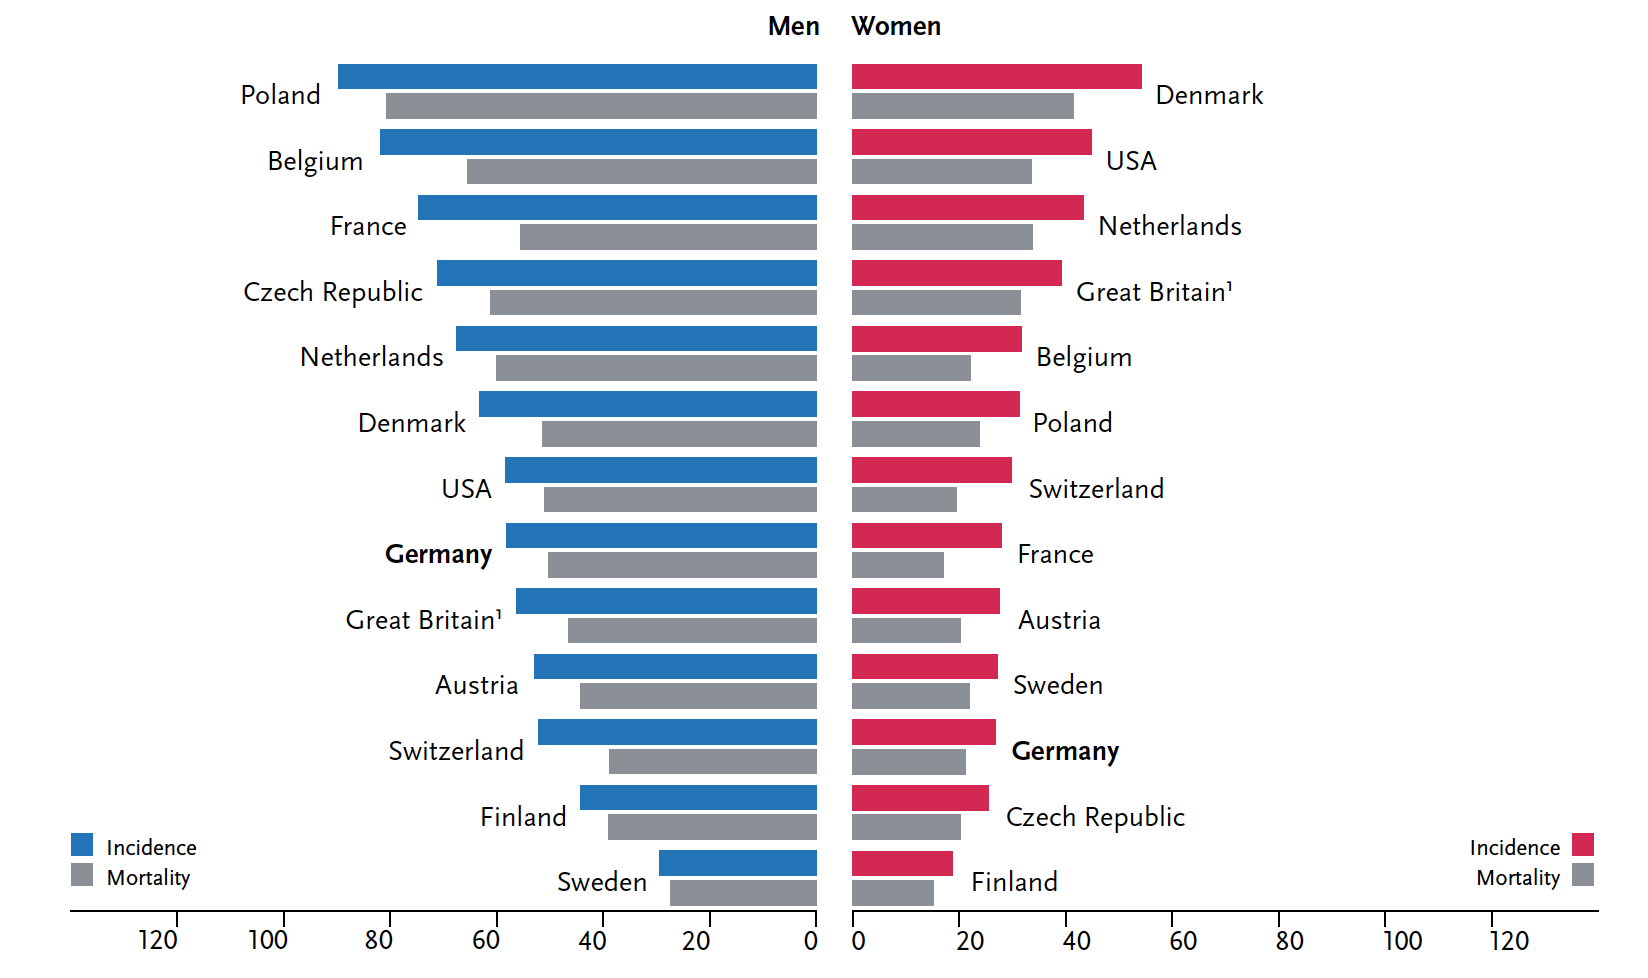
\includegraphics[width=\textwidth]{cancerInternational.png}
\caption{International comparison of age-standardized incidence and mortality rates for lung cancer in the year 2012}
\label{fig:cancInt}
\end{figure}

The main risk factor has been shown to be the exposure to tobacco smoke, whether it's active consumption via cigarettes, or passive exposure especially in closed rooms. CT scanners are used to detect irregular tissue in a patients lung region. These irregularities are grouped under the term \textit{pulmonary nodule}. A pulmonary nodule is a small, round (parenchymal) or worm (juxtapleural) shaped lesion in the lungs. Each lesion has a chance to be malignant and may grow and spread over time, becoming a risk for the patient's life in the form of lung cancer. Nodules come not only in different shapes but differ along other features as well. Ground-glass opacity (GGO) nodules are a challenging kind of nodules since they are not thoroughly solid and so harder to detect on a CT scan. The location of the nodules is crucial for the detection rate since nodules close to bigger vessels or the chest wall do not differ much in intensity to the surrounding tissue and can be easily overlooked by the radiologist.


\section{Current Medical Approach}
In the clinical setting, the supervising medical staff has additional information available apart from the CT scans. Patients are either in a high-risk group (over a certain age and heavy smokers) or present certain syndromes like fatigue, weight loss, cough, dyspnea, hemoptysis and chest pain. Different methods are used to find the underlying cause of these symptoms:

\begin{description}
\item[Sputum cytology] if patients cough up cells that can be used to check for irregularities in the lung tissue those can be used in analyzing the root of the illness
\item[Biopsy] taking samples from the irregular lung tissue
\item[Imaging tests] regular X-Ray vs CT vs LDCT 
\end{description}

Lung cancer is tricky to detect since the symptoms show up very late in the process of the illness and it is often too late for the patient when those are recognized. Sputum cytology and biopsy are only used when there is already circumstantial evidence (like other symptoms) for lung cancer which may often be too late in the development of the illness for a successful treatment. This makes imaging techniques the only source for early detection. Radiologists are required to analyze roughly 100-600 pictures per patient depending on the slice thickness of the used technique and the body height of the patient. Medical image viewers like OsiriX \ref{fig:osirix} are assisting in this process and have also been used in this thesis to analyze the image data.

\begin{figure}[ht]
\includegraphics[width=\textwidth]{Osirix_program.png}
\caption{Screenshot of the analyzing software OsiriX. It is the most widely used software in the domain of medical image viewers and offers a free trial version that was used for this thesis.}
\label{fig:osirix}
\end{figure}

Yet it is still a highly complicated task and despite all efforts in this field the process is of course not fail-safe and it can happen that nodules are not detected in an early stage of their development but later when a successful treatment is not as likely anymore. A study by Kakinuma et. al.     \cite{kakinuma2012comparison} shows how different features like the slice thickness and the nodule properties affect the detection rate, dropping it to 65.5$\%$ for pure ground-glass opacities in a scan with 2mm slice thickness. Another issue arises with the false positive rate. A study by Pinsky et. al.\cite{pinsky2013national} reports a mean false positive rate of 28.7$\%$ across 112 radiologists at 32 screening centers in and outside of the US. This puts additional stress on the patient and requires further tests to conclude that there is no cancer present.


\section{Opportunities for Assistance}

Early detection of lung cancer is important in two ways. First, it avoids unnecessary scans in the scenario of undetected cancerous material and it improves the error rate of radiologists.

There exist many algorithmic approaches to finding nodules in CT-Scans \cite{papers_classical} and some that make use of deep convolutional neural networks to solve related tasks \cite{papers_dnn}\\

Despite many effort being devoted to the computer-aided nodule detection problem, lung CAD systems remain an ongoing
research topic [18]. One of the major difficulties is the detection of GGO nodules with low-dose thin-slice CT screening. Another two difficulties are the detection of nodules that are adjacent to vessels or the chest wall when they have very similar density; and the detection of nodules that are nonspherical in shape. In such cases, intensity thresholding or model-based methods might fail to identify those nodules.

\section{Gaining insights from Deep Neural Networks}
Neural networks are strong tools that recently have been shown to solve all kind of problems. They can play computer games and drive a car, they can create new art and play go to name only a few examples. Yet it seems like the solution they come up with is not intelligible to humans. But in a scenario where medical decisions are based on the output of an algorithm, it is crucial that the algorithm is reliable and the way it comes up with a decision is accepted by the people responsible. As long as this is not the case it might still happen that the network produces erroneous results in some cases that did not occur during extensive training.

Strategies to cope with this problem include:
\begin{itemize}
\item Huge databases that contain a variety of samples. In this thesis, an open dataset is used that was
the result of a cooperative effort of many scientists and medical staff members and has proven
it's worth in many publications. A possible downside is still that the patients in this database are all Americans and that roughly 1000 patients are not enough to cover all possible cases.

\item Leaving the final decision up to a specialist. This makes sense in many automated processes that decide critical situations. The system is really rather assisting the decision maker. It could compensate a known shortcoming of the human detector or prepare the data in a way that speeds up the process of detection. The further advanced the automated assistance becomes the likelier it gets that the expert might rely too faithfully on it which may be troublesome if the system has built in biases stemming from the distribution of the data.
\end{itemize}

The main issue is that a neural network only remains to be a black box tool as long as no further insights into the problem can be gained through its solution. This is why this thesis is concerned with extracting features and solution mechanisms from a trained deep neural network on the example of lung CT data. If those extracted features are reasonable for solving the specific problem and they can be conceptualized in terms of already approved procedures, deep neural networks might really aid scientists in understanding novel approaches and solutions.

\section{Structure of this thesis}
This thesis is structured in the following way: in chapter \ref{chap:02data} the used dataset is described as well as it's preprocessing for the learning algorithm. The methods chapter (\ref{chap:03methods}) contains information about the used software packages that were necessary to implement the algorithms as well as information about convolutional neural networks and the learned model that is analyzed in chapter \ref{chap:04results}. That chapter focuses on extracting the features from the convolutional kernels and compares them to traditional approaches. In chapter \ref{chap:05discussion} the results are revised and items for further investigation and optimization are presented together with a more general outlook on the topic of analyzing neural networks to gain insights into problems and not just as solutions to them. 

\end{document}
